


\documentclass[
% serif,
% mathsans,
%  handout,
xcolor=dvipsnames, 
]
{beamer}
\usetheme{Pittsburgh}
\useinnertheme{circles}
\setbeamertemplate{enumerate items}[default]
\usecolortheme{rose}
\setbeamertemplate{navigation symbols}{}
  
\usefonttheme[butsansserifmath]{serif}

\setbeamertemplate{blocks}[rounded][shadow=false]
  
\usepackage[T1]{fontenc}
\usepackage[utf8]{inputenc}
\usepackage{verbatim}
\usepackage{csquotes}
\usepackage{graphicx}

\usepackage[charter,expert]{mathdesign}
\usepackage[scaled=.96,osf]{XCharter}
\linespread{1.04}

\usepackage{xspace}

\RequirePackage{xcolor}
\RequirePackage[color,all,2cell]{xy}\SelectTips{cm}{12}\SilentMatrices\UseAllTwocells

\usepackage{tikz}\usetikzlibrary{decorations.pathmorphing,arrows,decorations.text}

\newcommand{\plan}[1]{\textcolor{red}{#1}}

\definecolor{dkblue}{rgb}{0,0.1,0.5}
\definecolor{lightblue}{rgb}{0,0.5,0.5}
\definecolor{dkgreen}{rgb}{0,0.4,0}
\definecolor{dk2green}{rgb}{0.4,0,0}
\definecolor{dkviolet}{rgb}{0.6,0,0.8}

\newenvironment<>{goalblock}[1]{%
  \setbeamercolor{block title}{bg=Goldenrod!50!white}

  \begin{block}#2{#1}}{\end{block}}

\hypersetup{
colorlinks=true
}






\title{UniMath: its origins, present, and future}
\author{Benedikt Ahrens}
\date{}


\newcommand{\fat}[1]{\textbf{#1}}
\newcommand{\constfont}[1]{\ensuremath{\mathsf{#1}}}
\newcommand{\source}{\constfont{source}}
\newcommand{\target}{\constfont{target}}
\newcommand{\C}{\ensuremath{\mathcal{C}}}
\newcommand{\D}{\ensuremath{\mathcal{D}}}
\newcommand{\CC}{\ensuremath{\hat{\mathcal{C}}}}
\newcommand{\Set}{\constfont{Set}}
\newcommand{\Grp}{\constfont{Grp}}
\newcommand{\Rng}{\constfont{Rng}}
\newcommand{\ot}{\ensuremath{\leftarrow}}
\newcommand{\toiso}{\xrightarrow{\sim}}
\newcommand{\otiso}{\xleftarrow{\sim}}
\newcommand{\isIso}[1]{\ensuremath{\constfont{isiso}({#1})}}
\newcommand{\Iso}[2]{\ensuremath{\constfont{iso}({#1},{#2})}}
\newcommand{\sm}[2]{\ensuremath{\sum_{#1}{#2}}}
\newcommand{\isUniv}[1]{\ensuremath{\constfont{isUniv}({#1})}}
\newcommand{\idtoeq}{\constfont{idtoequiv}}
\newcommand{\eqtoid}{\constfont{equivtoid}}
\newcommand{\Path}{\constfont{Path}}
\newcommand{\Equiv}{\constfont{Equiv}}
\newcommand{\U}{\constfont{U}}
\newcommand{\Nat}{\constfont{Nat}}
\newcommand{\Bool}{\constfont{Bool}}
\newcommand{\Suc}{\constfont{Suc}}
\newcommand{\entails}{\ensuremath{ \enspace \vdash \enspace }}
\newcommand{\defined}{\ensuremath{\enspace\stackrel{\text{def}}{=}\enspace }}
\newcommand{\iso}{\constfont{iso}}
\newcommand{\comp}{\ensuremath{(\circ)}}
\newcommand{\RC}[1]{\ensuremath{\constfont{RC}({#1})}}
\newcommand{\GrpStructure}{\constfont{GrpStructure}}
\newcommand{\hProp}{\constfont{hProp}}
\newcommand{\isofhlevel}{\constfont{isofhlevel}}
\newcommand{\iscontr}{\constfont{iscontr}}
\newcommand{\isaprop}{\constfont{isaprop}}

\newcommand{\trans}[2]{\ensuremath{{#1}_{*}\mathopen{}\left({#2}\right)\mathclose{}}\xspace}
\let\Trans\trans
\newcommand{\transf}[1]{\ensuremath{{#1}_{*}}\xspace} % Without argument
\newcommand{\transfib}[3]{\ensuremath{\mathsf{transport}^{#1}(#2,#3)\xspace}}
\newcommand{\Transfib}[3]{\ensuremath{\mathsf{transport}^{#1}\Big(#2,\, #3\Big)\xspace}}
\newcommand{\transfibf}[1]{\ensuremath{\mathsf{transport}^{#1}\xspace}}





\newcommand{\spread}{\addtolength{\itemsep}{10pt}}


\newcommand{\outlinetitle}{Outline}

\AtBeginSection[]
{
  \begin{frame}<beamer>{\outlinetitle}
    \tableofcontents[currentsection]
  \end{frame}
}

\AtBeginSubsection[]
{
  \begin{frame}<beamer>{\outlinetitle}
    \tableofcontents[currentsection,currentsubsection]
  \end{frame}
}

\theoremstyle{definition}
\newtheorem{exercise}{Exercise}

\begin{document}




\begin{frame}
 \titlepage
\end{frame}

\begin{frame}
 \frametitle{\outlinetitle}
 \tableofcontents
\end{frame}

\section{Origins}

\begin{frame}
 \frametitle{Vladimir's interest in computer-checked proofs}
 
 \begin{quotation}
    PS I am thinking again about the applications of computers to pure
    math. Do you know of anyone working in this area? I mean mostly some
    kind of a computer language to describe mathematical structures, their
    properties and proofs in such a way that ultimately one may have
    mathematical knowledge archived and logically verified in a fixed
    format.
 \end{quotation}

 Email to Dan Grayson, Sept 2002
 
\end{frame}

\begin{frame}
 \frametitle{Vladimir's ideas about computer-checked proofs I}
  
  \begin{quotation}
    Let us start with what would be a perfect system of such sort [\ldots].

    Ideally one wants a math oracle. A user inputs a type expression and  
    the system either returns a term of this type or says that it has no  
    terms. The type expression may be ``of level 0'' i.e. it can correspond  
    to a statement in which case a term is a proof and the absence of  
    terms means that the statement is not provable. It may be ``of level  
    1'' e.g. it might be the type of solutions of an equation. In that  
    case the system produces a solution or says that there are non. It  
    may be ``of level 2'' e.g. It might be the type of all solvable groups  
    of order 35555. In that case the system produces an example of such a  
    group etc.

  \end{quotation}

 
\end{frame}

\begin{frame}
 \frametitle{Vladimir's ideas about computer-checked proofs II}
 \begin{quotation}
  A realistic approximation [\ldots] may look as follows.  
    Imagine a web-based system with a lot of users (both ``creators'' and  
    ``consumers'') and a very large ``database''.
    Originally the database is  
    empty (or, rather, contains only the primitive ``knowledge'' a-la  
    axioms). User A (say in Princeton) inputs a type expression and  
    builds up a term of this type either in one step (just types it in)  
    or in many steps  using the standard proof-assistant capabilities of  
    the system. Both the original and all the intermediate type  
    expressions which occur in the process are filed (in the real time)  
    in the database.  Enter user B (somewhere in Brazil), who inputs  
    another type expression and begins the process of constructing a term  
    of his type. 
 \end{quotation}

\end{frame}

\begin{frame}
 \frametitle{Vladimir's ideas about computer-checked proofs II}
 \begin{quotation}
    [\ldots]
    My homotopy lambda calculus is an attempt to create a system which is  
    very good at dealing with equivalences. In particular it is supposed  
    to have the property that given any type expression F(T) depending on  
    a term subexpression t of type T and an equivalence t->t' (a term of  
    the type Eq(T;t,t')) there is a mechanical way to create a new  
    expression F' now depending on t' and an equivalence between F(T) and  
    F'(T') (note that to get F' one can not just substitute t' for t in F  
    -- the resulting expression will most likely be syntactically  
    incorrect).
 \end{quotation}

   Email to Dan Grayson, Sept 2006
\end{frame}

\begin{frame}
 \frametitle{Vladimir learning how to use Coq}
 \begin{quotation}
    
 I am thinking a lot these days about foundations of math and automated proof
verification. My old idea about a ``univalent'' homotopy theoretical models of
Martin-Lof type systems survived the verification stage an I am in the
process of writing things up.

I also took a course at the Princeton CS department which was for most part
about Coq and was very impressed both by how much can be proved in it in a
reasonable time and by how many young students attended (45, 35 undergrad +
10 grad!). 

 \end{quotation}

   Email to Dan Grayson, Dec 2009

\end{frame}


\begin{frame}
 \frametitle{The Foundations library}
  
  In Feb 2010, Vladimir started writing the Coq library \emph{Foundations},
  making precise his ideas conceived during three years and collected in 
  \emph{A very short note on homotopy $\lambda$-calculus}.
  

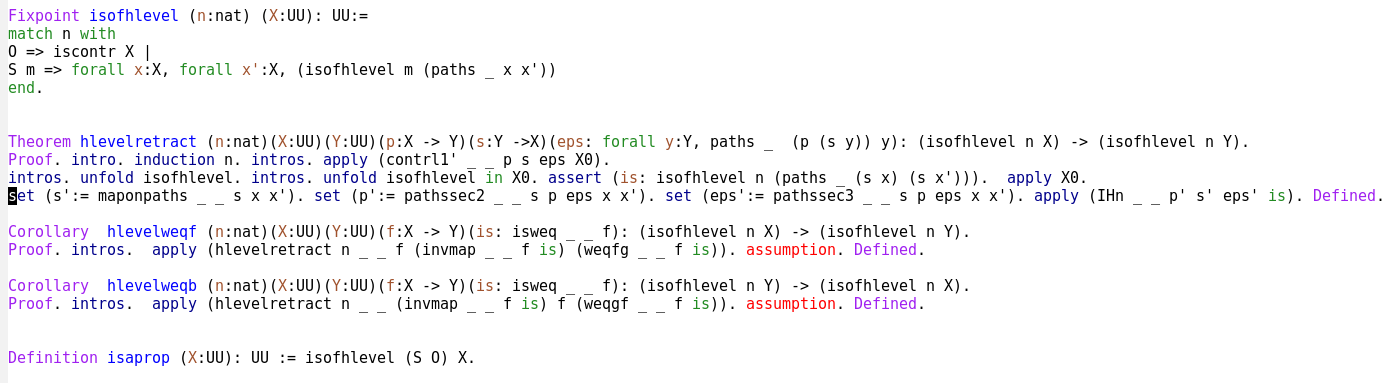
\includegraphics[width=\textwidth]{isofhlevel.png} 

Other libraries were built on top of \emph{Foundations}\ldots

\end{frame}
    
\begin{frame}
 \frametitle{Founding of UniMath}
 
 UniMath was founded in spring 2014, by combining three libraries:
 
 \begin{itemize}
  \item Foundations (Voevodsky) 
  \item RezkCompletion (Ahrens, Kapulkin, Shulman) (started Feb 2013)
  \item Ktheory (Grayson) (started Oct 2013)
 \end{itemize}

  A library on p-adic numbers, written by Pelayo, Warren, and Voevodsky in 2012, 
  was added to UniMath later as package \emph{PAdics}.
    
\end{frame}


\section{UniMath today}

\begin{frame}
 \frametitle{Some information on the UniMath library}
 
   \begin{itemize}
    \item ca.\ 120,000 loc
    \item Compile time: too long
    \item 15 contributors
    \item Distributed under free software license
   \end{itemize}

 
\end{frame}


\begin{frame}
 \frametitle{The UniMath library}
 
  Organized in `packages':
 \begin{itemize}
  \item Foundations 
  \item More Foundations
  \item Combinatorics
  \item Algebra
  \item Number Systems
  \item Real Numbers
  \item Category Theory
  \item Homological Algebra
  \item K-theory
  \item Topology
  
  \item \ldots
 \end{itemize}
\end{frame}




\begin{frame}
 \frametitle{Package Foundations}
 
   Provides a specification of ``univalent foundations'':
   
   \begin{itemize}
    \item Type and term constructors
    \item Definition of `weak equivalence'
    \item Definition of `h-level' for types and functions
    \item Facts on propositions and sets
    \item Univalence axiom and consequences
    \item Arithmetic on natural numbers
    \item \ldots
   \end{itemize}

 
  
\end{frame}


\begin{frame}
 \frametitle{Package MoreFoundations}

  Several variants of the same construction, e.g.,
  \begin{align*}  (a,b) = (a',b') \enspace & \simeq \enspace \sum_{p : a = a'} p_*(b) = b'  \\
                     t  = t'   \enspace & \simeq \enspace   \sum_{p : t.1 = t'.1} p_*(t.2) = t'.2
  \end{align*}

  useful, but not interesting---dilutes Foundations.
  
  Package MoreFoundations mirrors structure of Foundations:
  \begin{itemize}
   \item one variant of each construction in Foundations
   \item others in MoreFoundations
  \end{itemize}

  $\rightsquigarrow$ Foundations as a textbook on univalent foundations

\end{frame}

\begin{frame}
 \frametitle{Package Combinatorics}
 \begin{itemize}
  \item Standard finite sets
  \item Finite sets
  \item Finite sequences
  \item Ordered sets
  \item Wellordered sets
  \item Zermelo's wellordering theorem: 
        \\ AC $\Rightarrow$ every set can be well-ordered
 \end{itemize}

\end{frame}

\begin{frame}
 \frametitle{Package CategoryTheory}
 
 \begin{itemize}
  \item (Univalent) categories, functors, natural transformations
  \item Category of sets and Yoneda lemma
  \item Adjunctions, equivalences
  \item Rezk completion
  \item (Co)Limits in general, direct definition of some special (co)limits
  \item Abelian categories
  \item Displayed categories
  \item \ldots
 \end{itemize}

  
\end{frame}


\begin{frame}
  \frametitle{Package Algebra}
  \begin{itemize}
   \item Lattices
   \item Binary operations
   \item Monoids and groups, abelian groups
   \item Rigs and rings; 
   \item Ring of differences: construction of a (commutative) ring from a (commutative) rig (used to define the integers)
   \item Domains and fields
   \item Field of fractions: construction of a field from an integral domain with decidable equality (used to define the rationals)
   \item \ldots
  \end{itemize}

\end{frame}

\begin{frame}
 \frametitle{More specialized packages}
 
 \begin{itemize}
  \item Folds: categories via univalent FOLDS 
  \item Homological Algebra: 5-lemma for triangulated categories, naive homotopy category $K(A)$ is triangulated
  \item Ktheory: Torsors, the circle as $B(\mathbb{Z})$
  \item Number Systems: Integers and rationals via constructions in Algebra package
  \item SubstitutionSystems: theory of syntax with variable binding
  \item Tactics: tactics for proving results on monoids, groups, etc.
 \end{itemize}

\end{frame}


\section{The future of UniMath}

\subsection{Current issues}

\begin{frame}
 \frametitle{Propositional resizing}
 
  In a talk at TYPES 2011, Vladimir suggested a set of \fat{resizing rules}, in particular
  
  \begin{itemize}
   \item If type $A$ is a proposition, then $A$ lives in the lowest universe.
   \item For any universe $\U$, the type $\hProp(\U)= \sum_{X:\U}\isaprop(X)$ lives in the lowest universe.
  \end{itemize}


  Weakened versions of those rules---``up to equivalence''---are validated by Voevodsky's simplicial set model.
  
\end{frame}
  
\begin{frame}
  \frametitle{Use of resizing in UniMath}
  Propositional resizing is needed to achieve that
  \begin{itemize}
   \item the propositional truncation of $A$,
         \[
              |A| := \prod_{P : \hProp(\U)} (A \to P) \to P
         \]
lives in the same universe as $A$
   \item the set quotient of $(X,R)$ lives in the same universe as $X$;
         recall that elements of the quotient are equivalence classes $e : X \to \hProp(\U)$
  \end{itemize}
\end{frame}


\begin{frame}
 \frametitle{Research problems related to resizing}

 \begin{block}{Show consistency of resizing rules in univalent type theory}
    In the TYPES 2011 talk, Vladimir sketches a model of resizing that does not validate univalence.
 \end{block}

  \begin{block}{Implement a proof assistant with propositional resizing}
    \begin{itemize}
     \item In UniMath, resizing is currently achieved by the inconsistent rule $\U:\U$
     \item Dan Grayson is currently working on isolating the uses of $\U:\U$ into ``resizing modules''
    \end{itemize}

  \end{block}

\end{frame}

\subsection{Mathematical goals}

\begin{frame}
 \frametitle{What to work on?}
 
 \begin{itemize}
  \item UniMath aims to accommodate all of mathematics
  \item Anybody is welcome to contribute the mathematics they are interested in
  \item The purpose of this school/workshop has been to enable people to work on their own goals in UniMath
 \end{itemize}

 I am going to present some goals that have been suggested; you might pursue others!
  
\end{frame}


\begin{frame}
 \frametitle{Vladimir's goals for UniMath}
 
  In a lecture in July 2017, Vladimir outlined three goals for the UniMath library:
 
\end{frame}

\begin{frame}
 \frametitle{Vladimir's goals for UniMath I}
 ``
 The first direction is the development and formalization of the mathematics
surrounding the study of syntax and semantics of dependent type theories.

~\\

This direction itself has now branched into several subdirections. The most
clearly aimed among those is the one whose goal is to formalize the
construction of the univalent simplicial set model.

~\\

Its development progresses well.
''
\end{frame}

\begin{frame}
 \frametitle{Vladimir's goals for UniMath II}
 
 ``
 Another direction is the one that I have stated in my Bernays lectures at the
ETH in 2014 - to formalize a proof of Milnor’s conjecture on Galois
cohomology.

~\\

It has not been developing much. On the one hand, I discovered that
formalizing it classically it is not very interesting to me because I am quite
confident in that proof and in its extension to the Bloch-Kato Conjecture.

~\\

On the other hand, when planning a development of a constructive version of
this proof one soon encounters a problem. The proof uses the so called
Merkurjev-Suslin transfinite argument that relies on the Zermelo’s well-
ordering theorem that in turn relies on the axiom of choice for sets.
 ''
\end{frame}

\begin{frame}
 \frametitle{Vladimir's goals for UniMath III}
 
 ``
 Finally, there is the third direction that I think UniMath can and should develop.
It is the direction towards the modern theory of geometry and topology of
manifolds.

~\\

The first step in this direction can be a definition of a univalent category of
smooth manifolds. Univalence will force all the constructions relying on this
category to be invariant, or maybe better to say equivariant, with respect to
diffeomorphisms.

~\\

No one knows how much of the theory of smooth manifolds can be
developed constructively which creates an additional challenge.
'' 
\end{frame}




\begin{frame}
 \frametitle{UniMath for education}

  Make UniMath suitable for teaching
  
  \begin{itemize}
   \item type theory and univalent foundations
   \item mathematics
  \end{itemize}

 
 To this end:
  
  \begin{itemize}
   \item restrict use of tactics to a small, well-defined, set
   \item simplify installation
   \item improve documentation
   \item modernize user interface
   \item anything else? Suggestions welcome!
  \end{itemize}
 
\end{frame}


\begin{frame}
 \frametitle{Kudos to Coq}
 
  UniMath is a large codebase, with contributors coming and going.
  Its continued development would not be possible without the help of 
  Coq developers, who
  \begin{itemize}
   \item implement features useful for Foundations/UniMath
   \item ensure compatibility upon version upgrades
   \item test Coq with UniMath to check for regressions
   \item make Coq faster with every version 
  \end{itemize}

  
  
\end{frame}



\begin{frame}[fragile]
 \frametitle{References}
 \begin{itemize}
  \item Vladimir's emails to Dan Grayson \\ \url{https://groups.google.com/forum/#!topic/homotopytypetheory/K_4bAZEDRvE}
  \item Vladimir's library \emph{Foundations} \\ \url{https://github.com/vladimirias/Foundations}, archived at \url{https://github.com/UniMath/Foundations}
  \item Vladimir's talk at TYPES 2011 \\ \url{https://www.math.ias.edu/vladimir/sites/math.ias.edu.vladimir/files/2011_Bergen.pdf}
  \item Vladimir's talk on UniMath in July 2017 \\ \url{https://www.newton.ac.uk/seminar/20170710113012301}
 \end{itemize}

\end{frame}


\end{document}


